\documentclass[12pt]{amsart}
\setlength{\marginparwidth}{0.5in}
\usepackage{amsmath,amssymb,graphicx}
\textheight 9in
\textwidth 6.5 in
\hoffset -1 in
\voffset -1 in
\input FJHDef.tex

\newcommand{\sphere}{\mathbb{S}}
\newcommand{\cc}{\mathcal{C}}
\newcommand{\cq}{\mathcal{Q}}
\newcommand{\bbW}{\mathbb{W}}
\newcommand{\tP}{\widetilde{P}}
\newcommand{\bg}{{\bf g}}
\newcommand{\bu}{{\bf u}}
\newcommand{\bbu}{\bar{\bf u}}
\newcommand{\bv}{{\bf v}}
\newcommand{\bbv}{\bar{\bf v}}
\newcommand{\bw}{{\bf w}}
\newcommand{\bbw}{\bar{\bf w}}
\newcommand{\hv}{\hat{v}}
\newtheorem{theorem}{Theorem}
\newtheorem{prop}[theorem]{Proposition}
\begin{document}

\title{Adaptive Simple Monte Carlo}
\author{Fred J. Hickernell}
\author{Lan Jiang}
\author{Yuewei Liu}
\begin{abstract}We attempt a probabilistic analysis of simple Monte Carlo, achieving probabilistic error bounds when the kurtosis is controlled.  The algorithm uses a sample size that depends adaptively on the estimated variance of the integrand.  Thus, the algorithm is nonlinear (depending essentially on the function).  The advantage of what is done here over standard error analysis (complexity theory) is that the algorithm does not depend a priori on the scale of the problem (in this case the variance) to determine the number of samples.   Our intention, if what is done here is correct, is to try to extend this to the more sophisticated sampling schemes and infinite dimensional problems.
\end{abstract}
\maketitle

\section{Non-Adaptive Monte Carlo}
Suppose one wishes to compute the following integral or mean, $\mu$, of some function $g: \reals^d \to \reals$,
\begin{equation*}
\mu= \int_{\reals^d} g(\vx) f(\vx) \, \dif \vx,
\end{equation*}
where $f: \reals^d \to [0,\infty)$ is a probability density function.  The $\cl_{p,f}$ norm of $g$ is defined by
\[
\norm[p,f]{g} :=\left\{\int_{\reals^d} \abs{g(\vx)}^p f(\vx) \, \dif \vx\right\}^{1/p}
\]
Note that if $1 \le q<p$, then by H\"older's inequality,
\begin{align}\label{LP}
\norm[q,f]{g} &=\left\{\int_{\reals^d} \abs{g(\vx)}^q f(\vx) \, \dif \vx\right\}^{1/q}\\
\nonumber & \le \left\{\int_{\reals^d} \abs{g(\vx)}^p f(\vx) \, \dif \vx \right\}^{1/p} \left\{\int_{\reals^d} 1^{p/(p-q)} f(\vx) \, \dif \vx\right\}^{(p-q)/(pq)} \\
\nonumber & = \norm[p,f]{g} \norm[pq/(p-q),f]{1} = \norm[p,f]{g}.
\end{align}
Thus, $\cl_q \subseteq \cl_p$ for $1 \le q<p$.  As a consequence, if
\begin{equation} \label{momentdef}
M_p(g) := \int_{\reals^d} \abs{g(\vx)-\mu}^p f(\vx) \, \dif \vx, \qquad p \ge 1
\end{equation}
denotes the centered absolute moments of $g$, then
\begin{equation}\label{Mineq}
M_q \le M_p^{q/p} \quad \text{and} \quad M_p < \infty \implies M_q <\infty \qquad \text{for }1 \le q \le p.
\end{equation}

Let $\vX_1, \vX_2, \ldots$ be independent and identically distributed random variables with the probability density function $f$, briefly, $\vX_1, \vX_2, \ldots$ i.i.d.\ $\sim f$.  Then the simple Monte Carlo estimator of the mean, is
\begin{equation} \label{simpleMCest}
\hmu_n = \frac 1n \sum_{i=1}^n g(\vX_i).
\end{equation}
An important question that springs to mind is how to choose the right sample size, $n$, to achieve a specified tolerance, $\epsilon$.  The random estimator, $\hmu_n$ has mean $\mu$ and variance
\begin{equation*}
\var(\hmu_n) = \frac{\sigma^2}{n},
\end{equation*}
where $\sigma^2$ is the variance of the function $g$:
\begin{equation} \label{sigmadef}
\sigma^2 := \var(g) := M_2 = \int_{\reals^d} \abs{g(\vx)-\mu}^2 f(\vx) \, \dif \vx.
\end{equation}

In practice, one often invokes the Central Limit Theorem to determine sample size. Given a significance level or uncertainty tolerance, $\alpha$, one has
\[
\Prob\left[\abs{\hmu_n-\mu} \le \frac{z_{\alpha/2} \sigma}{\sqrt{n}} \right] \approx 1-\alpha.
\]
Thus one has the \emph{approximate} probabilistic result
\begin{equation} \label{CLTerr}
\Prob\left[\abs{\hmu_n-\mu} \le \epsilon \right] \approx 1-\alpha \qquad \text{for } n=N_{N}(\epsilon,\alpha,\sigma^2) :=\left \lceil \left(\frac{z_{\alpha/2}\sigma}{\epsilon}\right)^2 \right \rceil.
\end{equation}
The above is exact if $g(\vX_i)$ are i.i.d.\ normal, however, in general this result is only approximate and relies on the unknown $\sigma$.  The above observations are formalized in the proposition below.

\begin{prop} \label{nonadaptnormprop} For a given positive constant, $\sigma_{\max}$, define
\[
\cg_{2,N,\sigma_{\max}}= \{g \in \cl_{2,f} : g(\vX) \sim N(\mu,\sigma^2) \text{ for }\vX \sim f, \ \sigma^2 \le \sigma^2_{\max} \},
\]
where the variance of the function is defined in \eqref{sigmadef}.  If for a given error tolerance, $\epsilon$, and an uncertainty tolerance, $\alpha$, then a probabilistic error bound is given by
\[
\Prob\left[\abs{\hmu_n-\mu} \le \epsilon \right] \ge 1-\alpha \qquad \text{for } n \ge N_{N}(\epsilon,\alpha,\sigma_{\max}^2).
\]
\end{prop}

Note that the set $\cg_{2,N,\sigma_{\max}}$ assumes that $g(\vX)$ is normal, and that there is a priori knowledge about the variance of $g$.  The first of these drawbacks may be removed by turning to Chebyshev's inequality.

Using Chebyshev's inequality (Theorem \ref{Chebineqthm}) yields an exact upper bound rather than approximate one.  Choosing $Z=\hmu_n$ yields
\[
\Prob\left[\abs{\hmu_n-\mu} < \frac{\sigma}{\sqrt{n \alpha}} \right] \ge 1-\alpha.
\]
Thus, a proper choice of sample size guarantees that the estimate is within the tolerance of the true answer with probability $1-\alpha$:
\begin{equation} \label{Cheberr}
\Prob\left[\abs{\hmu_n-\mu} < \epsilon \right] \ge 1-\alpha \qquad \text{for } n= N_C(\epsilon,\alpha,\sigma^2):= \left \lceil \frac{\sigma^2}{\alpha\epsilon^2} \right \rceil.
\end{equation}
This sample size is typically much larger than $N_N$, since $1/\alpha$ is much larger than $z_{\alpha/2}^2$ as $\alpha \to 0$.  Figure \ref{alphacomparefig} compares these two quantities.

\begin{figure}
\centering
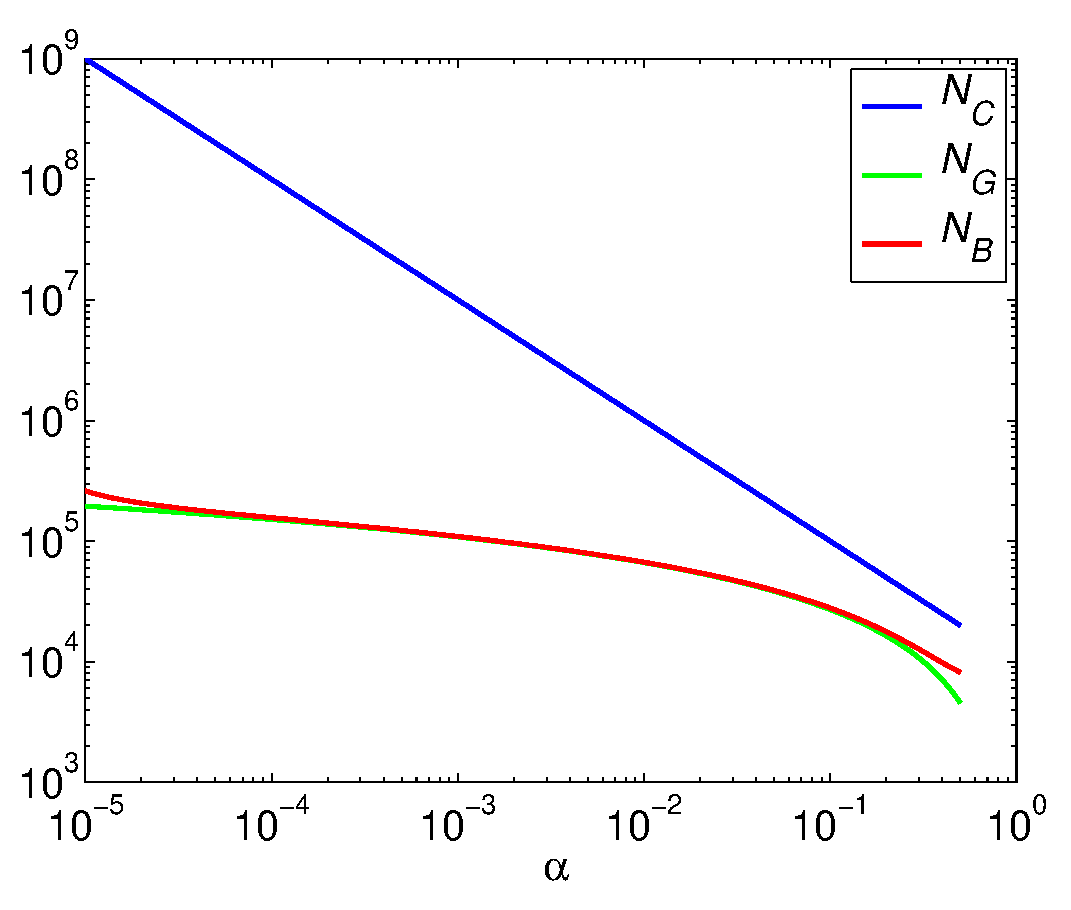
\includegraphics[width=3in]{alphacompare.eps}
\caption{Comparison of $N_N$, $N_C$, and $N_B$ for $\epsilon/\sigma = 0.001$, and $\rho=5$. \label{alphacomparefig}}
\end{figure}

\begin{prop} \label{nonadaptChebprop} For a given positive constant, $\sigma_{\max}$, define the set of functions
\[
\cg_{2,C,\sigma_{\max}}= \{g \in \cl_{2,f} : \var(g)= \sigma^2 \le \sigma^2_{\max} \},
\]
where the variance of the function is defined in \eqref{sigmadef}.  If for a given error tolerance, $\epsilon$, and an uncertainty tolerance, $\alpha$, then a probabilistic error bound is given by
\[
\Prob\left[\abs{\hmu_n-\mu} \le \epsilon \right] \ge 1-\alpha \qquad \text{for } n\ge N_{C}(\epsilon,\alpha,\sigma_{\max}^2).
\]
\end{prop}

A smaller sample size with a rigorous probabilistic bound can be
found by invoking the non-uniform Berry-Esseen inequality (Theorem
\ref{BE}). This inequality makes strong assumptions on the
distribution of $g(\vX)$, namely, a finite third moment:
\[
\varrho:=\frac{M_3}{\sigma^3} < \infty.
\]
Letting $Y_i = g(\vX_i)$, it follows that $\mu=E(Y_i)$ and $\hmu_n =
(Y_1 + \cdots + Y_n)/n$, and, furthermore, by the non-uniform
Berry-Esseen inequality,
\begin{align*}
\Prob\left[\abs{\hmu_n - \mu} <\frac{\sigma}{\sqrt{n}}x\right]&=\Prob\left[\hmu_n - \mu<\frac{\sigma}{\sqrt{n}}x\right]-\Prob\left[\hmu_n - \mu <-\frac{\sigma}{\sqrt{n}}x\right]\\
&\ge \left[\Phi(x)-A\frac{\varrho}{\sqrt{n}}(1+\abs{x})^{-3}\right] -\left[\Phi(-x) + A\frac{\varrho}{\sqrt{n}}(1+\abs{x})^{-3}\right]\\
&=1-2\left(A\frac{\varrho}{\sqrt{n}}(1+\abs{x})^{-3}+\Phi(-x)\right).
\intertext{Letting $\epsilon=\sigma x/\sqrt{n}$, the probability of
making a small error becomes} \Prob[\abs{\hmu_n -
\mu}<\epsilon]&\geq
1-2\left(A\frac{\varrho}{\sqrt{n}}\left(1+\frac{\epsilon\sqrt{n}}{\sigma}\right)^{-3}+\Phi\left(-\frac{\epsilon\sqrt{n}}{\sigma}\right)\right)\geq
1-\alpha,
\end{align*}
provided that $n$ is chosen to be larger than $N_B(\epsilon,\alpha,\sigma^2,\varrho)$, which is defined as the smallest integer satisfying
\begin{equation}\label{NB}
\Phi\left(-\frac{\sqrt{N_B}\epsilon}{\sigma}\right)+\frac{A\varrho}{\sqrt{N_B}}\left(1+\frac{\epsilon\sqrt{n}}{\sigma}\right)^{-3}
\le \frac{\alpha}{2}.
\end{equation}
This equation may be re-written as the implicit equation
\begin{equation}\label{NBalt}
N_B = \left \lceil \left(\frac{z_{\alpha/2 -  A
\varrho\sigma^3/\sqrt{N_B}(\sigma+\epsilon\sqrt{N_B})^3} \times
\sigma}{\epsilon}\right)^2 \right \rceil.
\end{equation}
\marginpar{check this}
The definition of $N_B$ implies that
\[
\max\left[\left(\frac{2A\varrho}{\alpha}\right)^2,N_N(\epsilon,\alpha,\sigma^2)
\right] \le N_B \le \max\left[ \left(\frac{2A
\rho}{\theta\alpha}\right)^2,
N_N(\epsilon,(1-\theta)\alpha,\sigma^2)  \right] , \quad 0 \le
\theta \le 1.
\]
As shown in Figure \ref{alphacomparefig}, $N_B$ is close to $N_N$ for moderate $\alpha$, but $N_B$ may be even larger than $N_C$ for very small $\alpha$.
\marginpar{end check}
\begin{prop} \label{nonadaptBerryprop} For given positive constants, $\sigma_{\max}$ and $\varrho_{\max}$, define the set of functions
\[
\cg_{3,B,\sigma_{\max},\varrho_{\max}}= \{g \in \cl_{3,f} : \var(g)= \sigma^2 \le \sigma^2_{\max}, \ M_3(g)/\sigma^3 \le \varrho_{\max} \},
\]
where the variance of the function is defined in \eqref{sigmadef}, and $M_3$ is defined in \eqref{momentdef}. If for a given error tolerance, $\epsilon$, an uncertainty tolerance, $\alpha$, then a probabilistic error bound is given by
\[
\Prob\left[\abs{\hmu_n-\mu} \le \epsilon \right] \ge 1-\alpha \qquad \text{for } n\ge N_{B}(\epsilon,\alpha,\sigma_{\max}^2,\varrho_{\max}),
\]
where $N_B$ is defined in $\eqref{NB}$.
\end{prop}

\section{Adaptive Monte Carlo}
Although the probabilitistic error results in Propositions \ref{nonadaptChebprop} and \ref{nonadaptBerryprop} based on the Chebyshev and Berry-Esseen inequalities are exact for general distributions, the classes of integrands are defined in terms of the typically unknown $\sigma^2=\var(g)$.  This is why in practice one typically uses observed function values observed to approximate the $\sigma^2$ by the sample variance, as follows:
\begin{equation} \label{samplevar}
\hv_{n} = \frac 1{n-1} \sum_{i=1}^{n} [g(\vX_i)- \hmu_{n}]^2.
\end{equation}
This means that we now have an \emph{adaptive} algorithm.  One might choose an initial sample of size $n_0$, and use it to estimate $\sigma^2$ by $\hv_{n_0}$.  Then one chooses an \emph{independent} sample of size $n=N_{N}(\epsilon,\alpha,\hv_{n_0})$, $n=N_{C}(\epsilon,\alpha,\hv_{n_0})$, or  $n=N_{B}(\epsilon,\alpha,\hv_{n_0},\varrho_{\max})$ or to compute $\hmu_n$ the final estimate of $\mu$.

Unfortunately, once we approximate $\sigma^2$ by $\hv_n$, we again have inexact results.  However, they can be made exact by using Cantelli's inequality (Theorem \ref{Can}) and the variance of $\hv_n$ in Theorem \ref{Varvarthm}.  Proposition \ref{propCant} implies that
\[
\Prob\left[\frac{\hv_n}{1 - \sqrt{\left ( \kappa  - \frac{n-3}{n-1}\right)\left(\frac{1-\alpha}{\alpha n}\right)}} > \sigma^2 \right] \ge 1 - \alpha,
\]
where
\begin{equation} \label{kurtdef}
\kappa:= \kurt(g) = \frac{M_4(g)}{\var^2(g)} = \frac{M_4(g)}{\sigma^4(g)} \ge 1
\end{equation}
denotes the \emph{kurtosis}.  Thus,
\begin{subequations}\label{probvarupbd}
\begin{gather}
\Prob\left[\hsigma_{\text{up}}(\hv_n,n,\alpha,\kappa)  > \sigma \right] \ge 1 - \alpha, \\
\text{where } \hsigma^2_{\text{up}}(\hv_n,n,\alpha,\kappa) = \frac{\hv_{n}}{1 - \sqrt{ \left ( \kappa  - \frac{n-3}{n-1}\right)\left(\frac{1-\alpha}{\alpha n }\right)}},
\end{gather}
\end{subequations}
provided that
\begin{align*}
1 &> \left ( \kappa  - \frac{n-3}{n-1}\right)\left(\frac{1-\alpha}{ \alpha n}\right)\\
\frac{\alpha n }{1-\alpha} & > \kappa  - \frac{n-3}{n-1} \\
\kappa & < \frac{\alpha n}{1-\alpha} + \frac{n-3}{n-1} =: \kappa_{\text{poss}} (\alpha,n).
\end{align*}

From another perspective, if we want the amplification factor to be smaller than $L$, i.e.,
\[
\frac{1}{1 - \sqrt{ \left ( \kappa  - \frac{n-3}{n-1}\right)\left(\frac{1-\alpha}{\alpha n }\right)}} \le L,
\]
then $n$ must be chosen to satisfy
\begin{gather*}
\left(\kappa  - \frac{n-3}{n-1}\right)\left(\frac{1-\alpha}{\alpha n }\right) \le \frac{L-1}{L}, \\
M\left[(\kappa-1)  + \frac{2}{n-1}\right] \le n, \qquad \text{where } M= \left(\frac{1-\alpha}{\alpha}\right)  \left(\frac{L}{L-1} \right), \\
(n-1)^2 - [(\kappa-1)M -1](n-1)  - 2 M \ge 0, \\
n \ge 1 + \frac{1}{2} \left\{ (\kappa-1)M -1 + \sqrt{\left[(\kappa-1)M -1\right]^2 + 8 M}\right\}.
\end{gather*}
Thus, for example, even in the best case scenario of $\kappa=1$, the smallest possible value, we have $n \ge [1 + \sqrt{1 + 8 M}]/2$.  For $L=2$ and $\alpha=0.05$ this translates into $M=38$ and $n \ge 9.2$.

\begin{theorem} \label{mainadaptthm} For a given positive constant, $\kappa_{\max}$, define the set of functions with bounded fourth moments:
\[
\cg_{4,\kappa_{\max}}= \{g \in \cl_{4,f} : \kurt(g)= \kappa \le \kappa_{\max} \},
\]
where the kurtosis of the function is defined in Theorem \ref{Varvarthm}.
Suppose that one has an error tolerance, $\epsilon$, and an uncertainty tolerance, $\alpha$. Let $\alpha_1 = 1 - \sqrt{1 - \alpha}$.  Pick any $n_0>1$ satisfying
\[
\kappa_{\max} < \kappa_{\text{\rm poss}}(\alpha_1,n_0)  = \frac{n_0 \alpha_1}{1-\alpha_1} + \frac{n_0-3}{n_0-1},
\]
and compute the sample variance, $\hv_{n_0}$ of a simple random sample of size $n_0$.   Use this to compute $\hsigma^2_{\text{\rm up}} = \hsigma^2_{\text{\rm up}}(\hv_{n_0},n_0,\alpha_1,\kappa_{\max})$ by \eqref{probvarupbd}.  Next choose an independent random sample of size
\[
n = \min\left( N_C(\epsilon,\alpha_1,\hsigma^2_{\text{\rm up}}), N_B(\epsilon,\alpha_1,\hsigma^2_{\text{\rm up}},\kappa_{\max}^{3/4}) \right)
\]
and compute $\hmu_n$, the simple Monte Carlo estimator of $\mu$.  Here $N_C$ is defined in \eqref{Cheberr} and  $N_B$ is defined in \eqref{NB}.  A probabilistic error bound is given by
\[
\Prob\left[\abs{\hmu_n-\mu} \le \epsilon \right] \geq 1-\alpha.
\]
\end{theorem}
\begin{proof}
By \eqref{probvarupbd} it follows that $\hsigma_{\text{up}}(\hv_{n_0},n_0,\alpha_1,\kappa)  \ge \sigma$ with probability $1-\alpha_1$.  By Propositions  \ref{nonadaptChebprop} and \ref{nonadaptBerryprop} it follows that  $\Prob\left[\abs{\hmu_n-\mu} \le \epsilon \right] \geq 1-\alpha_1$, provided that $\hsigma_{\text{up}}  \ge \sigma$.  Thus, the probability that both of these events happen, is at least $(1-\alpha_1)^2=1-\alpha$.
\end{proof}

The cost of this algorithm can be evaluated in a probabilistic way also.  Define the cost of an algorithm as the $1-\beta$ quantile of the total number of function evaluations:
\begin{equation}
\cost(\hmu_n(g),\beta) := \min\left\{M : \Prob(n_0 + n \le M) \ge 1-\beta  \right \}.
\end{equation}
Here, the cost is assumed to depend on the integrand, $g$.  For the algorithm described in Theorem \ref{mainadaptthm} we may derive an upper bound on the cost by means of Proposition \ref{propCant} as follows:
\begin{align*}
\lefteqn{\cost(\hmu_n(g),\beta)} \\
&= \min\left\{M : \Prob(n_0 + n \le M) \ge 1-\beta  \right \}\\
& = n_0 + \min\left\{M : \Prob\left( \min\left( N_C(\epsilon,\alpha_1,\hsigma^2_{\text{\rm up}}), N_B(\epsilon,\alpha_1,\hsigma^2_{\text{\rm up}},\kappa_{\max}^{3/4}) \right) \le M\right) \ge 1-\beta  \right \}.
\end{align*}
From form Proposition \ref{propCant} it follows that
\begin{align*}
1-\beta & \le \Prob\left[\hv_n < \sigma^2 \left\{1 + \sqrt{\left ( \kappa  - \frac{n-3}{n-1}\right)\left(\frac{1-\beta}{\beta n}\right)}\right\} \right] \\
& = \Prob\left[\frac{\hv_n} {1 - \sqrt{\left ( \kappa  - \frac{n-3}{n-1}\right)\left(\frac{1-\alpha_1}{\alpha_1 n}\right)}} < \sigma^2 \left\{\frac{1 + \sqrt{\left ( \kappa  - \frac{n-3}{n-1}\right)\left(\frac{1-\beta}{\beta n}\right)}} {1 - \sqrt{\left ( \kappa  - \frac{n-3}{n-1}\right)\left(\frac{1-\alpha_1}{\alpha_1 n}\right)}} \right\} \right] \\
& = \Prob\left[\hsigma^2_{\text{\rm up}}(\hv_{n_0},n_0,\alpha_1,\kappa_{\max}) < \sigma^2 \gamma(n_0,\alpha_1,\beta,\kappa_{\max}) \right],
\end{align*}
where,
\[
\gamma(n,\alpha_1,\beta,\kappa_{\max}) = \frac{1 + \sqrt{\left ( \kappa  - \frac{n-3}{n-1}\right)\left(\frac{1-\beta}{\beta n}\right)}} {1 - \sqrt{\left ( \kappa  - \frac{n-3}{n-1}\right)\left(\frac{1-\alpha_1}{\alpha_1 n}\right)}}.
\]
Since $N_C(\epsilon,\alpha_1, \cdot)$ and $N_B(\epsilon,\alpha_1, \cdot,\kappa_{\max}^{3/4})$ are increasing functions, it follows that
\begin{multline} \label{adaptcost}
\cost(\hmu_n(g),\beta) \le n_0 + \\
\min\left( N_C(\epsilon,\alpha_1,\var(g)\gamma(n_0,\alpha_1,\beta,\kappa_{\max})), N_B(\epsilon,\alpha_1,\var(g)\gamma(n_0,\alpha_1,\beta,\kappa_{\max}),\kappa_{\max}^{3/4}) \right).
\end{multline}

\begin{theorem} \label{costtheorem} The algorithm described in Theorem \ref{mainadaptthm} has a probabilistic cost given by \eqref{adaptcost}.
\end{theorem}

The key factors that determine $\cost(\hmu_n(g),\beta)$ are $\epsilon$, the error tolerance, and $\var(g)$.  The cost is roughly proportional to $\var(g)\epsilon^{-2}$.  For the set of integrands $\cg_{4,\kappa_{\max}}$ the variance, $\var(g)$ is unbounded.  Thus, the cost is not bounded, however, it does seem to behave as expected as a function of the variance of the integrand.  As mentioned before, this is actually an advantage of this analysis.  One need not make any assumptions about the variance of the integrand, only about the kurtosis, which is unchanged when the integrand is multiplied by an arbitrary constant.

%Consider a spacial case in (\ref{NB}), let $\Phi(-\frac{\sqrt{n}\epsilon}{\sigma})=\frac{A\varrho}{\sqrt{n}}=\frac{\alpha}{4}$, since $\varrho\leq (\kappa_{\max}+3)^{3/4}$,
%we can get the upper bound of $N_B(\epsilon,\alpha_1,\sigma_{\max},\varrho)$ by
%$$N_B(\epsilon,\alpha_1,\sigma_{\max},\varrho)\leq \max\{\frac{Z^2_{\alpha_1/4}\sigma^2_{\max}}{\epsilon^2},\frac{16A^2(\kappa_{\max}+3)^{3/2}}{\epsilon^2}\}$$

\section{Example}

Consider the case of the uniform probability distribution on $[0,1]$, i.e., $f=1$.  Define
\begin{equation} \label{exampleeq}
g(x) = \begin{cases} 1 + \sigma \sqrt{\frac{1-p}{p}}, & 0 \le x \le p,\\
1 - \sigma \sqrt{\frac{p}{1-p}}, & p < x \le 1,
\end{cases}
\end{equation}
where $p$ and $\sigma$ are parameters, with $0 < p < 1$.
Note that
\begin{align*}
\mu &= \int_0^1 g(x) \, \dif x = 1\\
\var(g) &= \int_0^1 [g(x)-\mu]^2 \, \dif x = \sigma^2 \frac{1-p}{p} p + \sigma^2 \frac{p}{1-p} (1-p) = \sigma^2, \\
\kappa = \kurt(g) &= \frac{1}{\sigma^4}\int_0^1 [g(x)-\mu]^4 \, \dif x = \left(\frac{1-p}{p}\right)^2 p + \left(\frac{p}{1-p} \right)^2 (1-p) \\
& = \frac{(1-p)^3 + p^3}{p(1-p)} = \frac{1-3p+3p^2}{p(1-p)} = \frac{1}{p(1-p)} - 3.
\end{align*}
Note that $\kappa$ ranges from a minimum of $1$, when $p=1/2$ to a maximum of $\infty$ when $p=0,1$.

\begin{figure}
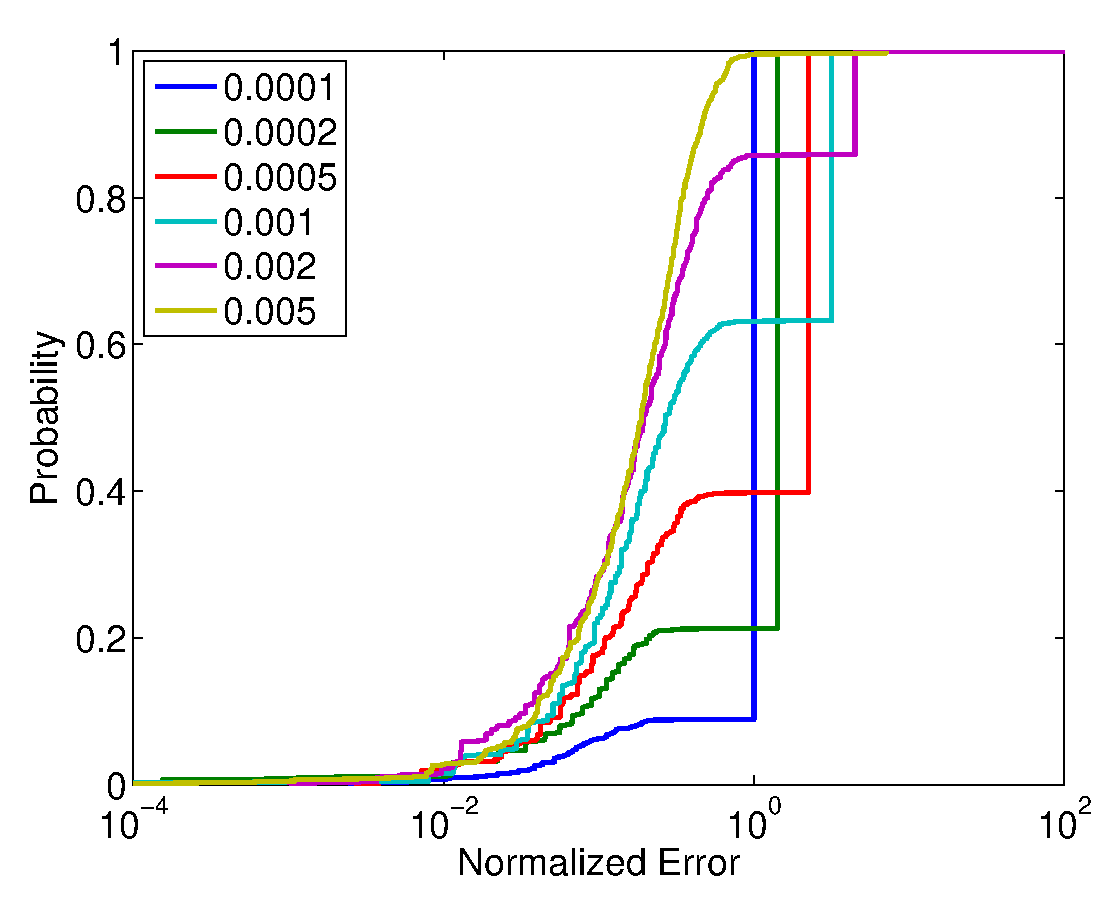
\includegraphics[width=3in]{NormalErrFig.eps}
\caption{Empirical distribution function of $\abs{\mu-\hmu_n}/\epsilon$ for example \eqref{exampleeq} with $\mu=\sigma=1$, $n_0=100$, $\kappa_{\max} = 3.2$, $\epsilon=0.01$, and  $p=0.001, 0.002, 0.005, 0.01, 0.02, 0.05$ using the algorithm in Theorem \ref{mainadaptthm}. \label{normalerrfig}}
\end{figure}

Figure \ref{normalerrfig} shows the empirical distribution of the normalized error $\abs{\mu-\hmu_n}/\epsilon$, using $1000$ replications for a range of values of $p$.  As can be seen in this figure and in Table \ref{examptable}, the adaptive Monte Carlo method does poorly for very small values of $p$, which correspond to vary large values of the kurtosis.  However, even for values of the kurtosis above $\kappa_{\max}=3.2$ used in this example, the chance of meeting the error tolerance may be quite high.

\begin{table}
\caption{Kurtosis probability of meeting the error tolerance for different values of $p$. \label{examptable}}
\[
\begin{array}{r|ccccccccccc}
p &   0.001 &    0.002 &    0.005 &     0.01 &     0.02 &     0.05 \\
\hline
\kappa &  998.00 &   498.00 &   198.01 &    98.01 &    48.02 &    18.05 \\
\hline
\Prob(\abs{\mu-\hmu_n} \le \epsilon) &    8.70\% &    17.50\% &    39.20\% &    63.50\% &    86.40\% &    99.90\% \\
\end{array}
\]
\end{table}


\section{Questions}

Here are some questions that suggest themselves:

\begin{itemize}

\item Is this analysis above known already?  Is this the typical probabilistic setting?  Is it better to look at a randomized setting where one considers the expected value of the error?

\item Can this type of analysis be extended to randomized \emph{quasi-Monte Carlo} for finite dimension, $d$?  Infinite dimension?  In this latter case one needs some multilevel algorithm, but the specification of the levels perhaps could be deduced from the data.  One might also consider a case where the coordinate weights were not known a priori but needed to be estimated.

\item Is there already this kind of information-based complexity analysis where the number of operations is bounded above or below by the unknown scale of the problem (in this case the variance).  The IBC I know assumes that the scale is fixed, e.g., the function has variance one, norm one, etc.  Here we allow arbitrary scale, but do make assumptions on the nastiness (kurtosis).

\item Are there better inequalities than Chebyshev's inequality or the Berry-Esseen inequality that apply when $Z$ is the sum of i.i.d.\ random variables?  Some of the better known ones, like Hoeffding's inequality assume boundedness, which we cannot presume here.

\end{itemize}

\section*{Appendix}
\begin{theorem}[Chebyshev's Inequality] \label{Chebineqthm} Let $Z$ be any random variable with mean $\mu$ and variance $\sigma^2$.  Then for all $\alpha >0$, Chebyshev's inequality states that
\[
\Prob\left[\abs{Z-\mu} \ge \frac{\sigma}{\sqrt{\alpha}} \right] \le \alpha, \qquad \Prob\left[\abs{Z-\mu} < \frac{\sigma}{\sqrt{\alpha}} \right] \ge 1-\alpha.
\]
\end{theorem}
\begin{proof}To prove Chebyshev's inequality note that
\begin{equation*}
\sigma^2 = E[\abs{Z-\mu}^2] \ge \frac{\sigma^2}{\alpha} \Prob\left[\abs{Z-\mu} \ge \frac{\sigma}{\sqrt{\alpha}} \right],
\end{equation*}
and then divide both sides by $\sigma^2/\alpha$.
\end{proof}
Theorem 5.16 in \cite{p1}
\begin{theorem}[Non-uniform Berry-Esseen Inequality] \label{BE} Let $Y_1,\dots,Y_n$ be i.i.d.\ random variables.  Suppose that
\[
\mu=E(Y_i), \quad \var(Y_i)=\sigma^2>0, \quad \varrho=\frac{E\abs{Y_i - \mu}^3}{\sigma^3} < \infty.
\]
Then
\[
\abs{\Prob\left[\frac{1}{\sigma\sqrt{n}}\sum_{i=1}^{n}(Y_i-\mu)<x
\right]-\Phi(x)}\leq \frac{A \varrho}{\sqrt{n}}(1+\abs{x})^{-3}.
\] for all x,
where $\Phi$ is the cumulative distribution function of the standard normal random variable, and $A$ is some number satisfying $0.4097\leq A\leq 0.5600$.
\end{theorem}

\begin{theorem} \label{Varvarthm} Let $\hv_n$ be the sample variance as defined in \eqref{samplevar}.  It's variance is
\[
\var(\hv_n^2) = \frac{\sigma^4}{n} \left ( \kappa  - \frac{n-3}{n-1} \right),
\]
where $\kappa:= \kurt(g) = M_4(g)/\sigma^4(g)$ denotes the \emph{kurtosis}.
\end{theorem}
\begin{proof}The sample variance has mean $\sigma^2/n$.  To facilitate the derivation, let $Y_i=g(X_i) - \mu$.
\begin{align*}
\hv_n & =  \frac 1{n-1} \sum_{i=1}^n \left[Y_i- \left(\frac 1n \sum_{j=1}^n Y_j\right) \right]^2
=  \frac 1{n(n-1)}\left[ n \sum_{i=1}^n Y^2_i-  \sum_{j,k=1}^n Y_jY_k \right] \\
\hv_n^2 & = \frac 1{n^2(n-1)^2}\left[ n^2 \sum_{i,j=1}^n Y^2_i Y^2_j  - 2 n \sum_{i,j,k=1}^n Y^2_i Y_j Y_k +  \sum_{i,j,k,l=1}^n Y_iY_j Y_k Y_l\right] \\
E[ Y^2_i Y^2_j] & = \begin{cases} M_4, & i=j,\\
\sigma^4, & i \ne j,
\end{cases}\\
\sum_{i,j=1}^n E[Y^2_i Y^2_j]&= n M_4 + n(n-1)\sigma^4, \\
E[ Y^2_i Y_j Y_k] & = \begin{cases} M_4, & i=j=k,\\
\sigma^4, & i \ne j, j=k,\\
0, & j \ne k,
\end{cases} \\
\sum_{i,j,k=1}^n E[Y^2_i Y_j Y_k] &= nM_4  + n(n-1)\sigma^4 \\
E[ Y_i Y_j Y_k Y_l] & = \begin{cases} M_4, & i=j=k=l,\\
\sigma^4, & i, j, k, l \text{ have 2 distinct values},\\
0, & \text{otherwise},
\end{cases}\\
\sum_{i,j,k,l=1}^n E[Y_iY_j Y_k Y_l] &= n M_4 + 3n(n-1)\sigma^4 \\
E[\hv_n^2] & = \frac{ n^3[M_4 + (n-1)\sigma^4]  - 2 n^2 [M_4 + (n-1)\sigma^4] +  n[M_4 + 3(n-1)\sigma^4]} {n^2(n-1)^2} \\
& = \frac{ (n-1)M_4 + (n^2-2n+3)\sigma^4} {n(n-1)} \\
\var(\hv_n^2) & = E[\hv_n^2] - \left[E(\hv_n)\right]^2 = \frac{ (n-1)M_4 + (n^2-2n+3)\sigma^4} {n(n-1)} -\sigma^4\\
& = \frac{(n-1)M_4 + (-n+3)\sigma^4} {n(n-1)}= \frac{1}{n} \left ( M_4 - \frac{n-3}{n-1} \sigma^4 \right) = \frac{\sigma^4}{n} \left ( \kappa  - \frac{n-3}{n-1} \right).
\end{align*}
\end{proof}
\begin{theorem}[Single tailed Cantelli's inequality]\label{Can}
Let $Z$ be any random variable with mean $\mu$ and finite variance $\sigma^2$.  For any $a\geq 0$, it
follows that:
\[
\Prob[Z-\mu \geq a]\leq \frac{\sigma^2}{a^2+\sigma^2}.
\]
\end{theorem}
\begin{proof}Define the random variable
\[ S=\sign(Z - \mu - a) = \begin{cases} 1, & Z - \mu \geq a,\\ -1, & Z - \mu <a. \end{cases}
\]
From conditional probability it is known that
\begin{align*}
\sigma^2 &= \var(Z-\mu)=E[\var(Z-\mu|S)]+\var[E(Z-\mu|S)] \\
&\geq\var[E(Z-\mu|S)]= E[\{E(Z-\mu|S)\}^2]-[E\{E(Z-\mu|S)\}]^2 =  E[\{E(Z-\mu|S)\}^2]
\end{align*}
Since $E(Z-\mu)=0$, it follows that
\begin{equation*}
0= E[E(Z-\mu|S)]=E(X|S=1)\Prob(Z - \mu \geq a)+E(X|S=-1)\Prob(Z - \mu < a).
\end{equation*}
Also, it is clear that $E(Z - \mu|S=1) \ge a$, which implies that
\begin{equation*}
[E(Z - \mu|S=-1)]^2=\left[\frac{E(Z - \mu|S=1)\Prob(Z - \mu \geq a)}{\Prob(Z - \mu < a)}\right]^2\geq \left[\frac{a\Prob(Z - \mu \geq a)}{\Prob(Z - \mu < a)}\right]^2
\end{equation*}
Combining these results together yields
\begin{align*}
\sigma^2 & \ge E[\{E(Z-\mu|S)\}^2]\\
& =\{E(Z-\mu|S=1)\}^2 \Prob(Z - \mu \geq a) + \{E(Z-\mu|S=-1)\}^2 \Prob(Z - \mu < a) \\
& \ge a^2 \Prob(Z - \mu \geq a) + \left[\frac{a\Prob(Z - \mu \geq a)}{\Prob(Z - \mu < a)}\right]^2 \Prob(Z - \mu < a) \\
&= a^2 \left[\frac{ \Prob(Z - \mu \geq a)}{\Prob(Z - \mu < a)}\right] = a^2 \left[\frac{ \Prob(Z - \mu \geq a)}{1  - \Prob(Z - \mu \ge a)}\right]
\end{align*}
Solving this inequality for $\Prob(Z - \mu \geq a)$ completes the proof.
\end{proof}

\begin{prop}\label{propCant} Let $\hv_n$ be the sample variance of a function $g$ as defined in \eqref{samplevar}, and let $\kappa=\kurt(g)$.  Then
\begin{subequations} \label{sampvarbd}
\begin{gather}\label{sampvarup}
\Prob\left[\hv_n < \sigma^2 \left\{1 + \sqrt{\left ( \kappa  - \frac{n-3}{n-1}\right)\left(\frac{1-\alpha}{\alpha n}\right)}\right\} \right] \ge 1 - \alpha, \\
\label{sampvarlo}
\Prob\left[\hv_n > \sigma^2 \left\{1 - \sqrt{\left ( \kappa  - \frac{n-3}{n-1}\right)\left(\frac{1-\alpha}{\alpha n}\right)}\right\} \right] \ge 1 - \alpha.
\end{gather}
\end{subequations}
\end{prop}
\begin{proof}Choosing
$$a=\sigma^2\sqrt{\left(\kappa-\frac{n-3}{n-1}\right)\left(\frac{1-\alpha}{\alpha n}\right)} >0,
$$
we know from Cantelli's inequality (Theorem \ref{Can})  that
$$\Prob[\hv_n-\sigma^2 \geq
a]\leq\frac{\var(\hv_n)}{a^2+\var(\hv_n)}$$
\begin{align*}
\Prob\left[\hv_n-\sigma^2 \geq
\sigma^2\sqrt{\left(\kappa-\frac{n-3}{n-1}\right)\left(\frac{1-\alpha}{\alpha n}\right)} \right] & = \Prob\left[\hv_n-\sigma^2 \geq
a \right]\\
& \leq\frac{\var(\hv_n)}{a^2+\var(\hv_n)}\\
&= \frac{\frac{\sigma^4}{n}\left(\kappa - \frac{n-3}{n-1}\right)}{\frac{\sigma^4}{n}\left(\kappa - \frac{n-3}{n-1}\right)\left(\frac{1-\alpha}{\alpha}\right)+\frac{\sigma^4}{n}\left(\kappa - \frac{n-3}{n-1}\right)} \\
&=\frac{1}{\left(\frac{1-\alpha}{\alpha}\right)+1}=\alpha.
\end{align*}
Then \eqref{sampvarup} follows directly.  By a similar argument.
\begin{align*}
\Prob\left[\hv_n-\sigma^2 \le
- \sigma^2\sqrt{\left(\kappa-\frac{n-3}{n-1}\right)\left(\frac{1-\alpha}{\alpha n}\right)} \right] & = \Prob\left[\hv_n-\sigma^2 \le -a \right]\\
& = \Prob\left[(-\hv_n)-(-\sigma^2) \ge a \right]\\& \leq\frac{\var(-\hv_n)}{a^2+\var(-\hv_n)}= \frac{\var(\hv_n)}{a^2+\var(\hv_n)}\\
&= \frac{\frac{\sigma^4}{n}\left(\kappa - \frac{n-3}{n-1}\right)}{\frac{\sigma^4}{n}\left(\kappa - \frac{n-3}{n-1}\right)\left(\frac{1-\alpha}{\alpha}\right)+\frac{\sigma^4}{n}\left(\kappa - \frac{n-3}{n-1}\right)} \\
&=\frac{1}{\left(\frac{1-\alpha}{\alpha}\right)+1}=\alpha.
\end{align*}
Thus, \eqref{sampvarlo} follows as well.
\end{proof}

\begin{thebibliography}{99}
\bibitem{p1}Valentin V. Petrov, \emph{Limit Theorems of Probability Theory:Sequences of Independent Random Variables},
Clarendon press,Oxford, 1995,P168.
\end{thebibliography}
\end{document}
